
\subsection{Cross-Dimensional Knowledge Projection and Pressure-Prior Construction}
\label{sec:knowledge-projection}

The pretrained sectional baseline and regional correction models provide complementary aerodynamic knowledge for target-wing pressure prediction. The sectional model supplies the baseline pressure response at each spanwise section, whereas the root- and tip-region models provide localized finite-span corrections. Because the regional models are trained on constant-chord source configurations, their positional inputs cannot be transferred directly to target wings with varying local chord lengths and planform shapes. To address this discrepancy, the target wing is first represented sectionwise, and the source-domain knowledge is then queried through cross-dimensional mapping to construct a three-dimensional pressure prior, as illustrated in Fig.~\ref{fig:hierarchical-prior-construction}.

For a target wing with spanwise-varying geometry, let $z$ denote the physical spanwise coordinate measured from the wing root, $b_h$ the semispan, and $c(z)$ the local chord length. Each target-wing section is represented by its local airfoil geometry and flow conditions and is evaluated independently by the pretrained sectional baseline model. To establish a spanwise positional representation that is transferable across wings with different chord distributions, the cumulative chord-count coordinates measured from the root and tip are defined as
\begin{equation}
\begin{aligned}
q_r(z) &= \int_0^z \frac{\mathrm{d}\zeta}{c(\zeta)},\\
q_t(z) &= \int_z^{b_h} \frac{\mathrm{d}\zeta}{c(\zeta)}.
\end{aligned}
\label{eq:integrated-chord-coordinates}
\end{equation}
For a constant-chord wing, these coordinates reduce to the corresponding root- and tip-distances normalized by the chord length. They therefore provide a common spanwise-position measure for evaluating the pretrained regional correction models on target wings with different planform scales and taper ratios.

In addition to spanwise-position mapping, local flow matching is introduced to improve the consistency between the source-domain knowledge queries and the target-wing conditions. For the target-domain dataset, the sectional Reynolds number is determined from the freestream Mach number and the local chord length as $Re(z)=8.1166\times10^6 M_\infty c(z)$, where $c(z)$ is expressed in meters. To account for the stronger influence of leading-edge sweep near the wing root, the sweep condition supplied to the pretrained knowledge models is replaced by a spanwise-dependent effective sweep angle:
\begin{equation}
\Lambda_{\mathrm{eff}}(z)
=
\Lambda_{c/4}
+
\left(\Lambda_{\mathrm{LE}}-\Lambda_{c/4}\right)
\exp\left(-\frac{z}{L_{\Lambda}c_r}\right),
\label{eq:effective-sweep-mapping}
\end{equation}
where $\Lambda_{\mathrm{LE}}$ and $\Lambda_{c/4}$ are the geometric leading-edge and quarter-chord sweep angles, respectively, $c_r$ is the root chord, and $L_{\Lambda}=0.5$ defines the transition length in root-chord units. For a trapezoidal planform, the leading-edge sweep angle is obtained from
\[
\tan\Lambda_{\mathrm{LE}}
=
\tan\Lambda_{c/4}
+
\frac{1-\lambda}{AR(1+\lambda)},
\]
where $AR$ and $\lambda$ denote the aspect ratio and taper ratio. The effective sweep approaches the leading-edge value near the root and the quarter-chord value away from the root, thereby improving the local flow correspondence without changing the target-wing geometry itself.

Using the mapped flow variables and spanwise coordinates, the frozen source-domain knowledge models are evaluated sectionwise on the target wing. The sectional baseline model provides $\widehat{C}_{p,s}^{\mathrm{sec}}$, while the root- and tip-region correction models provide $\widehat{\Delta C}_{p,r,s}$ and $\widehat{\Delta C}_{p,t,s}$, respectively. To avoid extrapolation beyond the spatial ranges represented in the source-domain training data, the positional queries used by the regional models are clipped to their valid training ranges. The unclipped chord-count coordinates are retained for the subsequent spatial weighting of the predicted regional corrections.

Because the root- and tip-region corrections represent localized finite-span effects, their contributions should decay with increasing distance from the corresponding wing boundaries. A monotonic gating function is therefore introduced for each region:
\begin{equation}
g_j(q_j)
=
\frac{
\operatorname{sigmoid}\left[k_j(L_j-q_j)\right]
}{
\operatorname{sigmoid}(k_jL_j)
},
\qquad j\in\{r,t\},
\label{eq:regional-gating}
\end{equation}
where $L_j$ and $k_j$ control the effective range and decay steepness of the regional correction. The root and tip regions use separate gating parameters, while the upper and lower surfaces share the same spatial gating function within each region.

The hierarchical pressure prior is constructed by combining the sectional baseline prediction with the gated regional corrections:
\begin{equation}
\begin{aligned}
C_{p,s}^{\mathrm{prior}}(z,\xi)
={}&
\widehat{C}_{p,s}^{\mathrm{sec}}(z,\xi)
+
a_{r,s}g_r\!\left[q_r(z)\right]\widehat{\Delta C}_{p,r,s}(z,\xi)
+
a_{t,s}g_t\!\left[q_t(z)\right]\widehat{\Delta C}_{p,t,s}(z,\xi),
\end{aligned}
\qquad s\in\{u,l\},
\label{eq:hierarchical-pressure-prior}
\end{equation}
where $a_{r,s}$ and $a_{t,s}$ are surface-specific amplitude factors for the root- and tip-region corrections, respectively. These factors are initialized by ridge-regularized least-squares calibration using only the target-domain training samples and are constrained within prescribed bounds. During the initial stage of target-domain residual learning, the gating and amplitude parameters are held fixed; they are subsequently refined jointly with the residual model at a reduced learning rate, while all pretrained source-domain knowledge models remain frozen.

Through this cross-dimensional projection and fusion procedure, the sectional baseline response and localized finite-span corrections learned from source-domain data are combined into a three-dimensional surface-pressure prior for the target wing. This prior provides the initial pressure estimate and serves as the main aerodynamic guidance for the subsequent target-domain residual learning described in Sec.~\ref{sec:target-residual}.

\begin{figure*}[t]
    \centering
    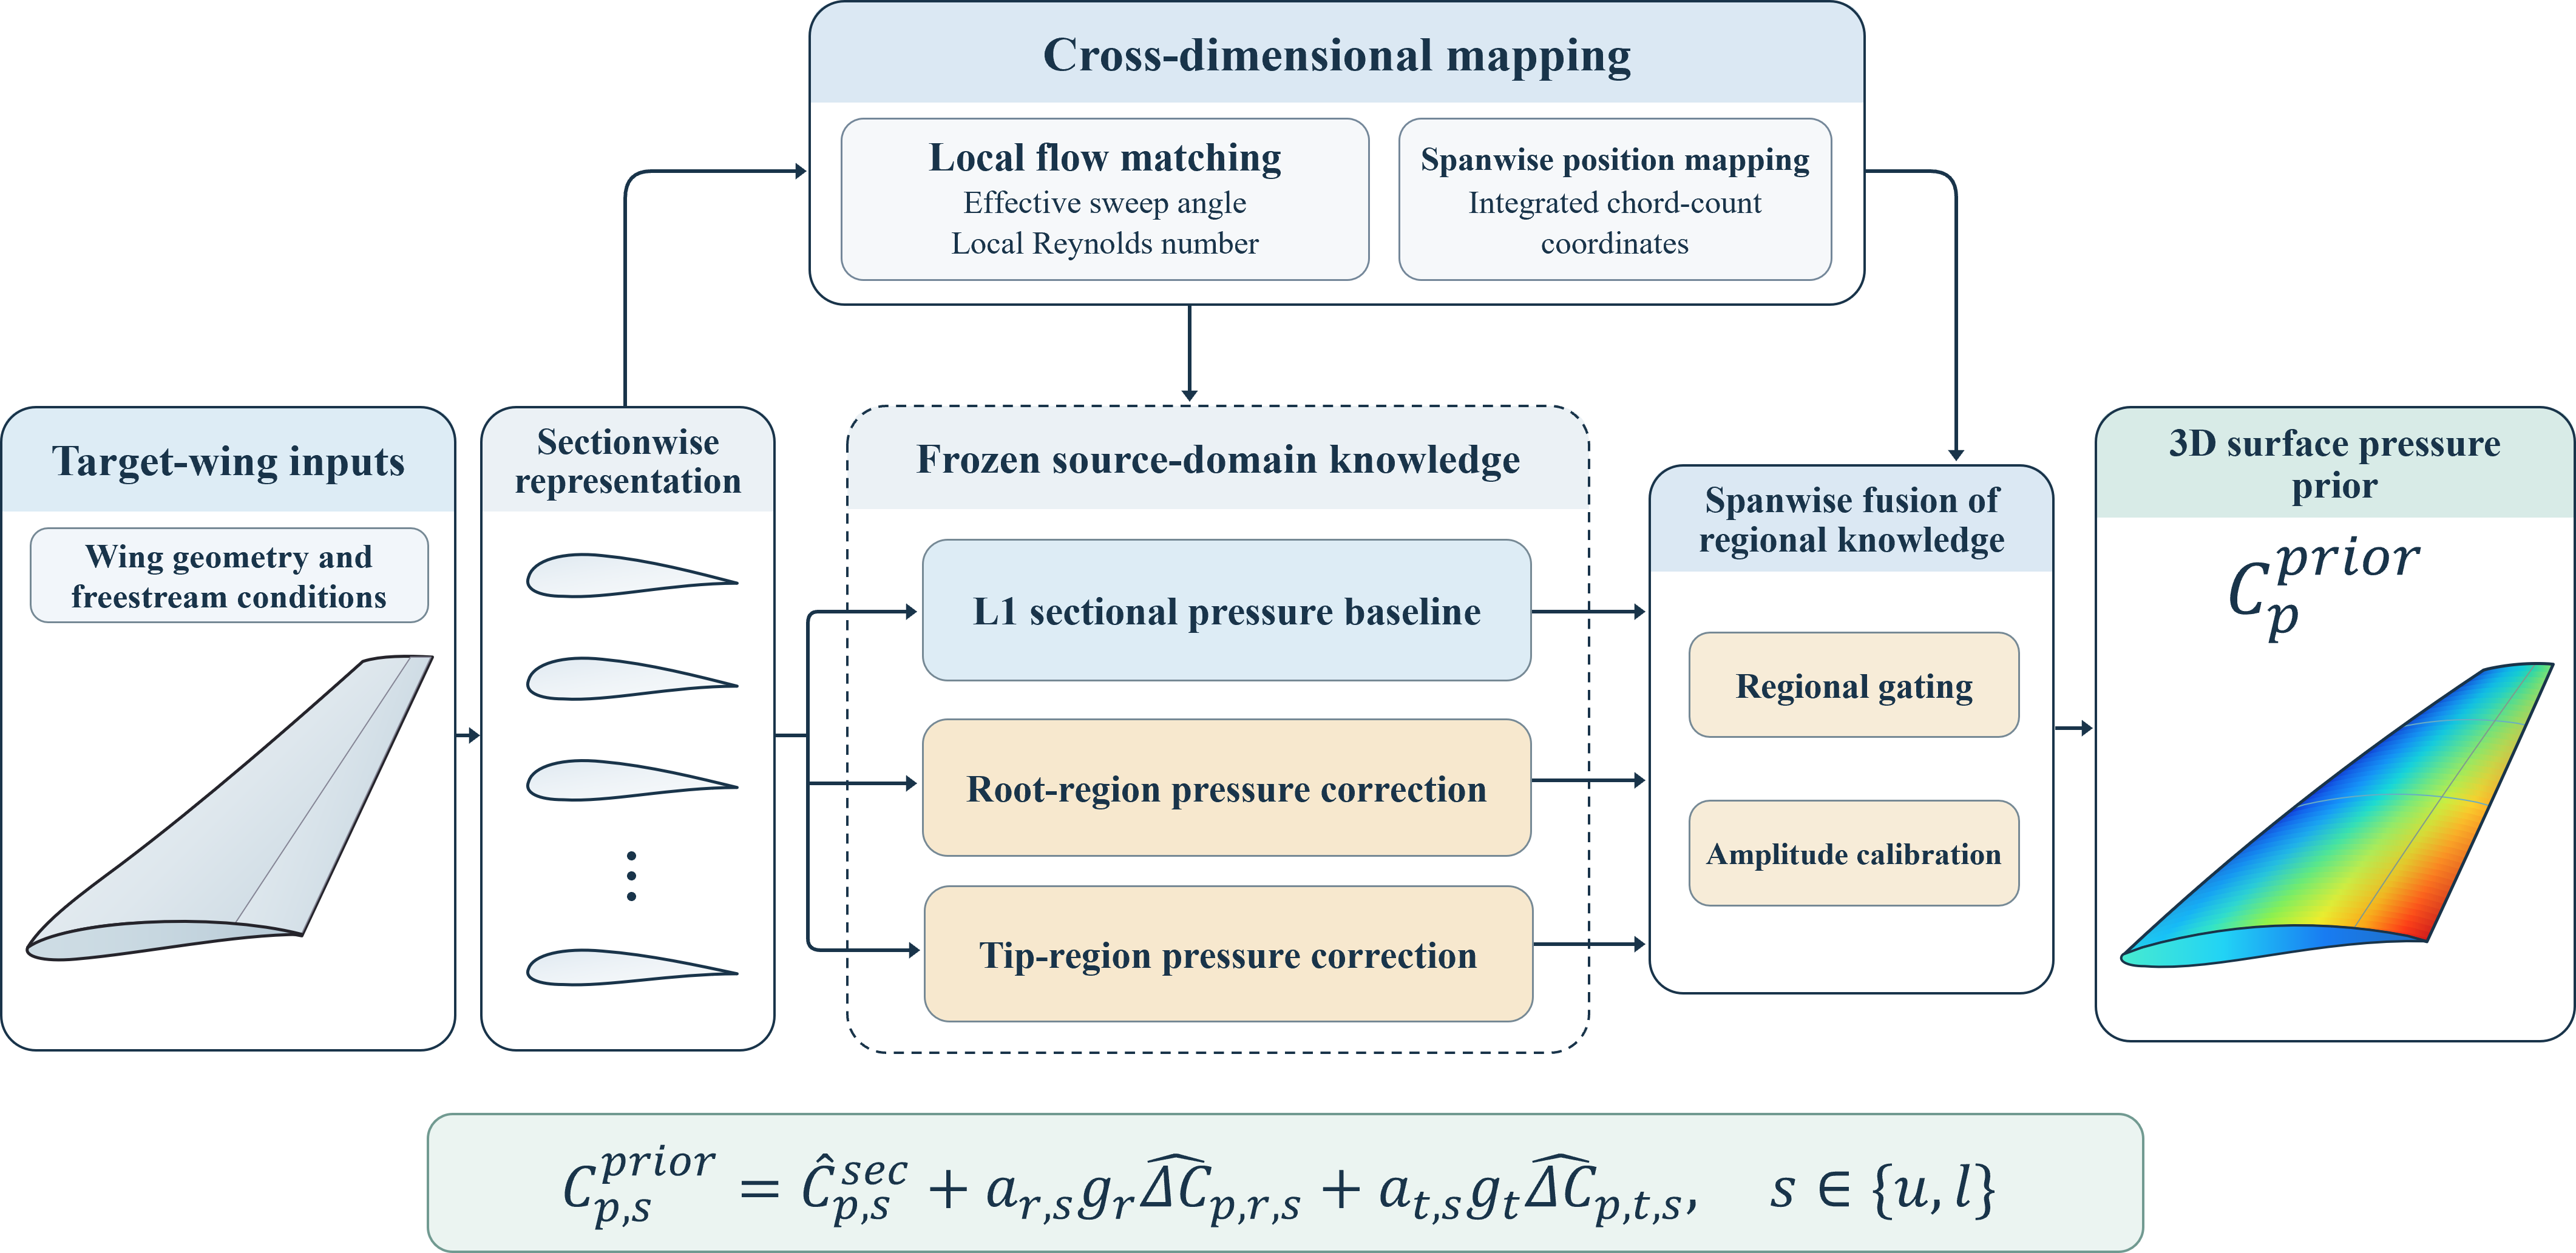
\includegraphics[width=0.98\textwidth]{III_Knowledge_Transfer/figures/III_C_Fig11/III_C_Fig11_hierarchical_prior_construction.png}
    \caption{Cross-dimensional knowledge projection and hierarchical pressure-prior construction for target-wing surface-pressure prediction.}
    \label{fig:hierarchical-prior-construction}
\end{figure*}